\newpage
\section{Anhang}
\subsection{Anhang 1}
\label{sec:Anhang1}
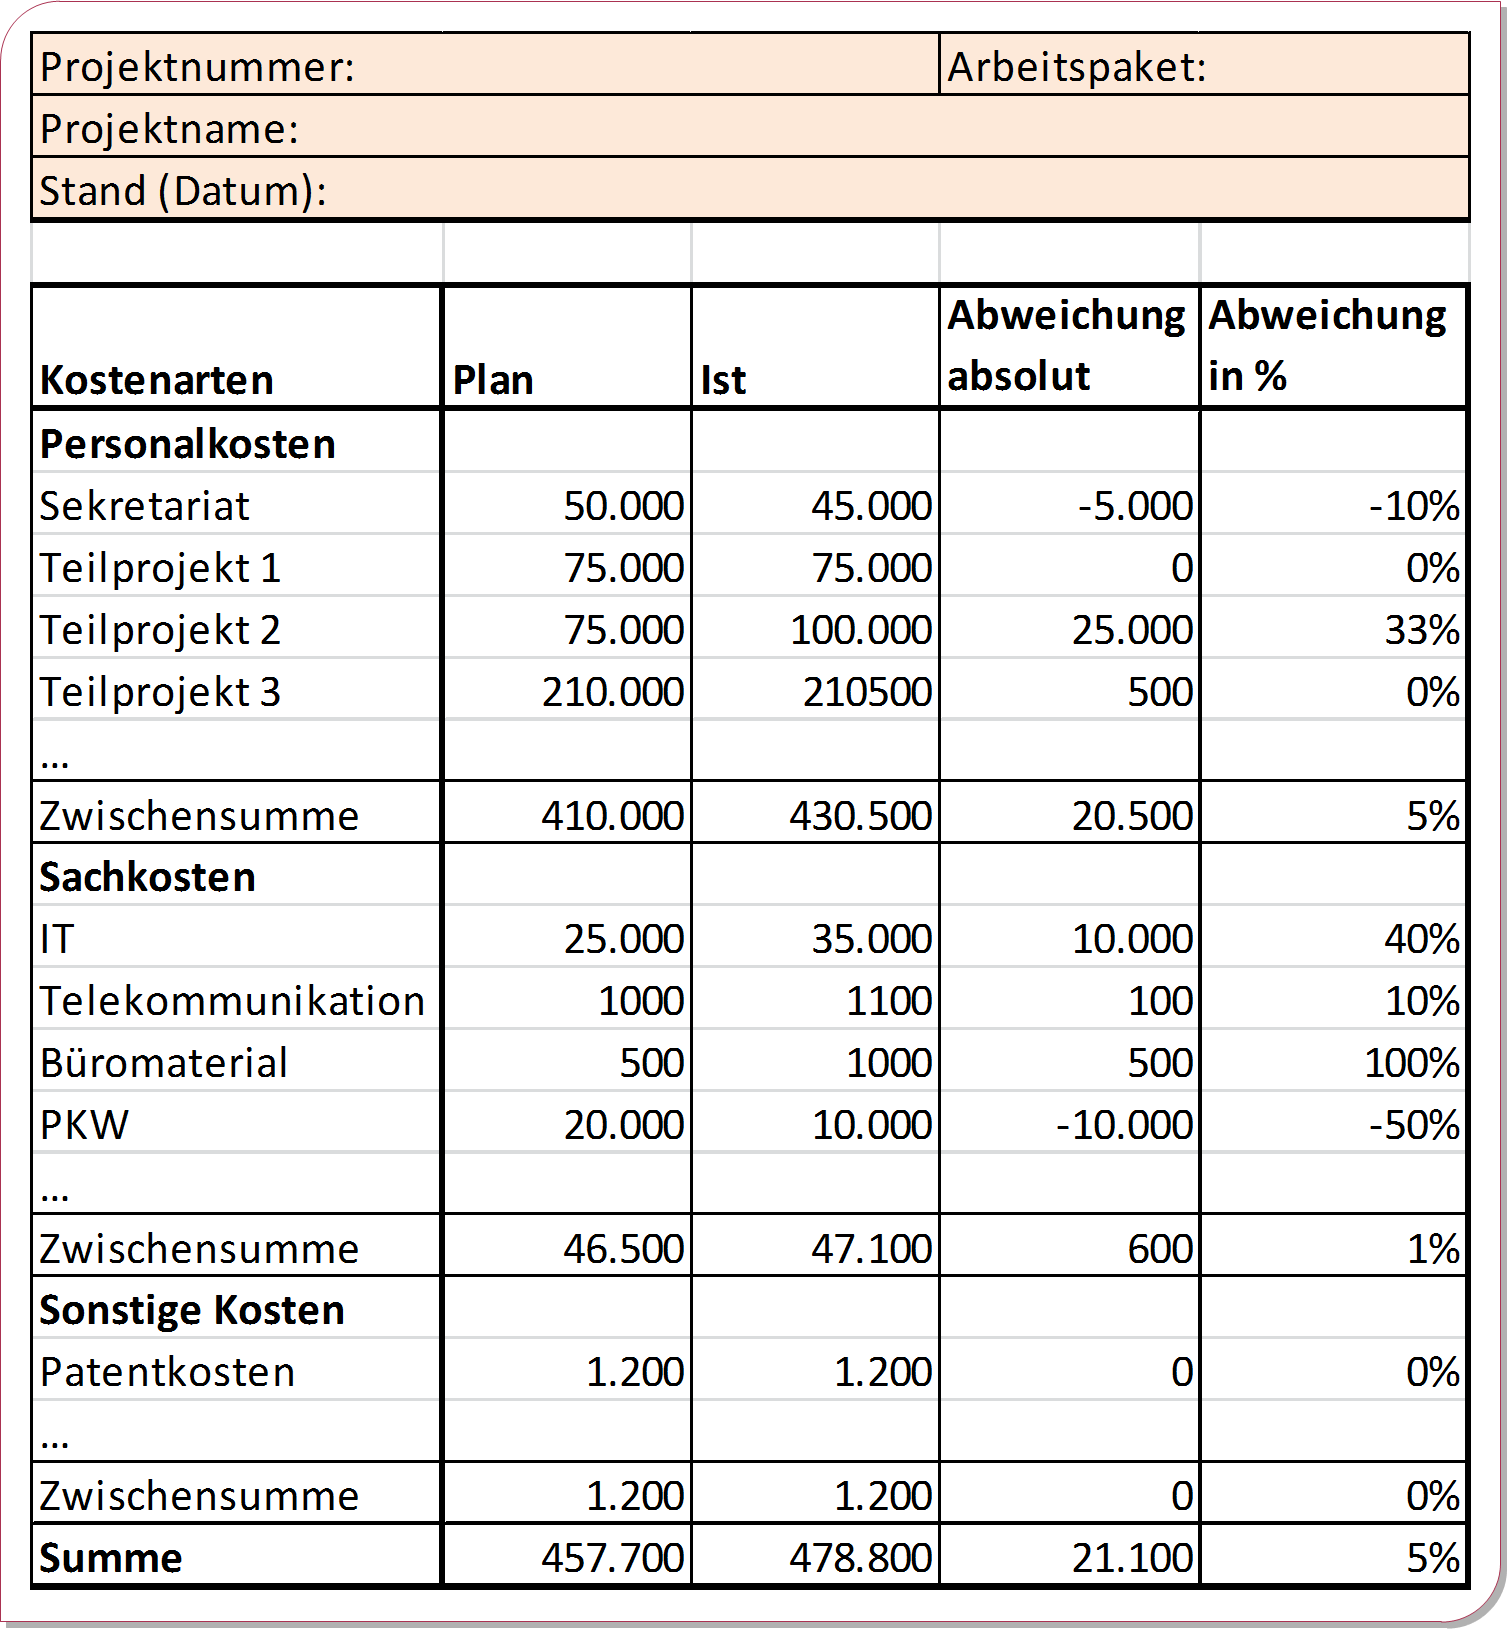
\includegraphics[width=1\textwidth]{Images/PlanIstVergleich.png} 
\begin{center}
   {\footnotesize In Anlehnung an: \cite{Blazek2001}, S. 137}\\
   Einfacher Plan-Ist-Vergleich
   %   \caption[Einfacher Plan-Ist-Vergleich]{Einfacher Plan-Ist-Vergleich}\label{abb3}
\end{center}
%\end{figure}
%\end{floatingfigure}
\newpage
\subsection{Anhang 2}
\label{sec:Anhang2}
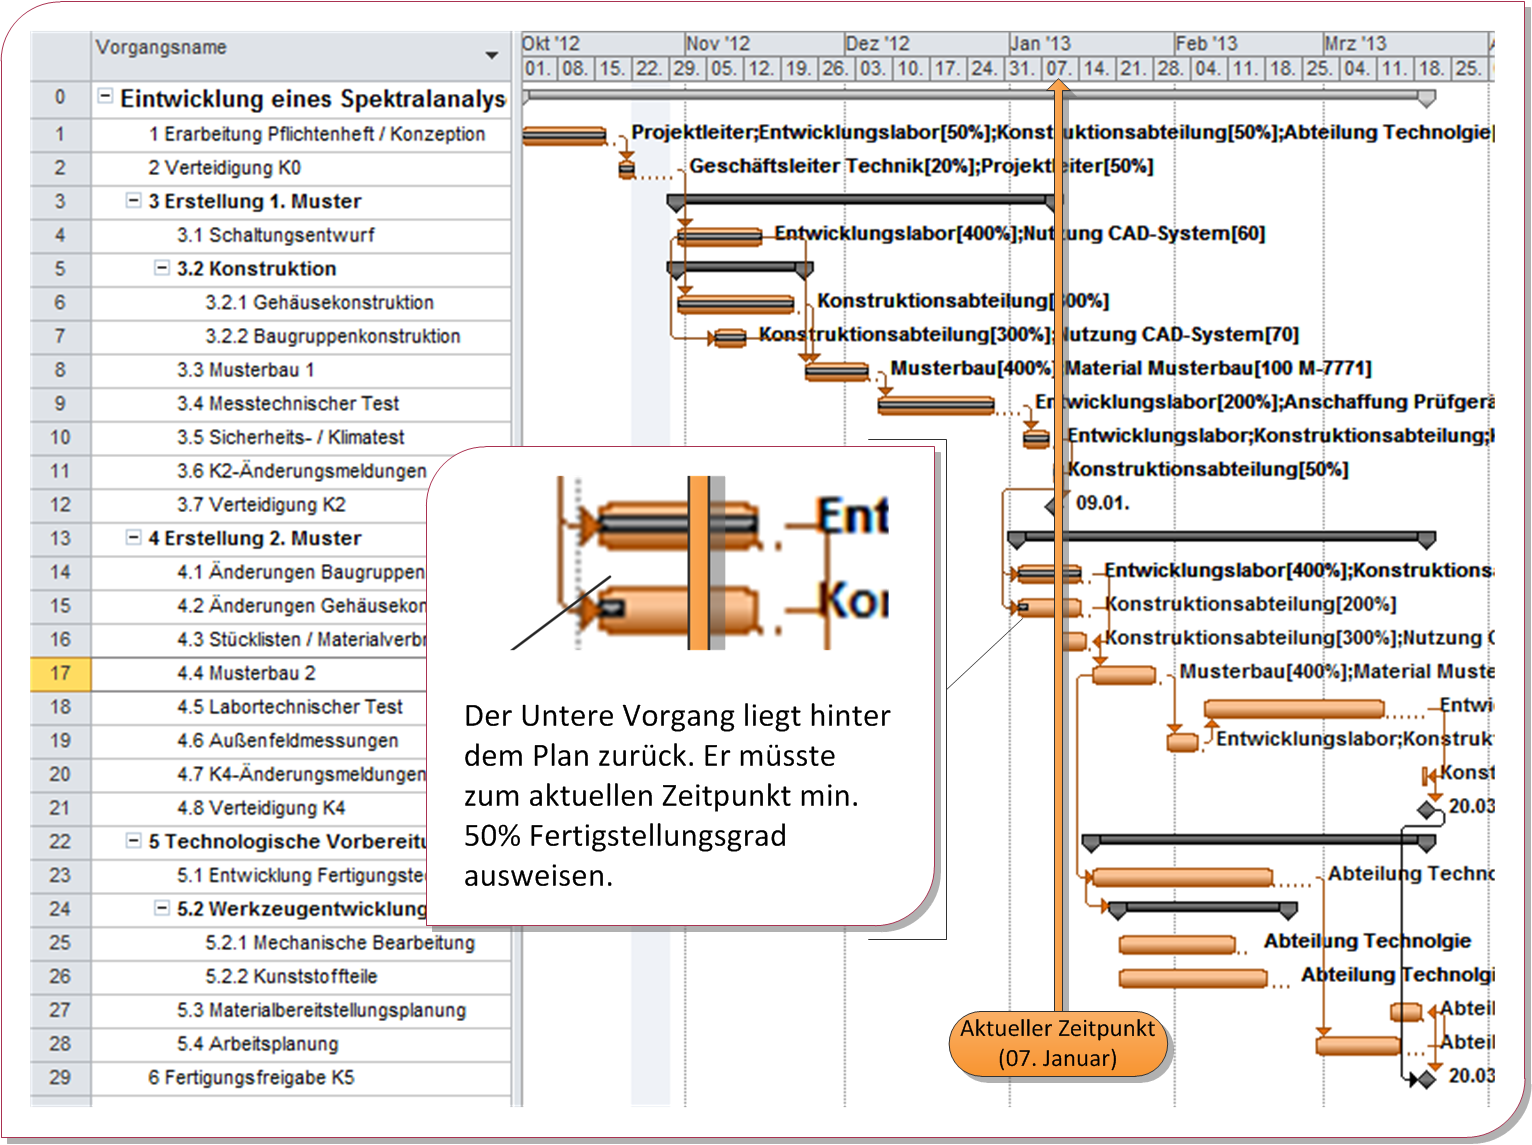
\includegraphics[width=1\textwidth]{Images/MSPfortschritt.png} 
\begin{center}
   %{\footnotesize In Anlehnung an: \cite{Blazek2001}, S. 137}\\
   Projektfortschrittsbericht in MS-Project
   %   \caption[Einfacher Plan-Ist-Vergleich]{Einfacher Plan-Ist-Vergleich}\label{abb3}
\end{center}
%\end{figure}
%\end{floatingfigure}
\newpage